% Drawing 151/01-2 -- folder 151, batch 01, archive page 19 (PDF page 20).
% Transcription: au bas de la page, au milieu, quatre figures griffonnées, sans lettres. À gauche : trois points entourés d'un ovale (les deux premiers encadrés), trois autres points au-dessous entourés d'un second ovale, et trois boucles étroites obliques joignant ceux du haut à ceux du bas. À droite : deux points encadrés et un troisième à côté, le tout entouré d'un ovale ; au-dessous, deux points entourés d'un ovale. Plus bas : un segment épais à deux points marqués, dont la partie droite est encadrée.
% Kind: scribbled figures: marked points grouped by ovals and frames (count of fixed points). Method 2 (schematic redraw from the facsimile). Status: partial.
% Notes: Right: a frame round two points and a third point beside it, all three inside an oval; below, two points inside an oval. Bottom: a heavy segment with two marked points, a frame round its right part (the right point is inside the frame). Left: three points in an oval, a frame round the first two; three points below in a second oval; three narrow oblique loops (spindles) from above the upper row down to the lower row. Still differs: the left figure is scribbled over itself; which points each narrow loop contains is a reading (drawn as the page shows them: the first round the second upper point and the first lower point, the second round the third upper point and the second lower point, the third, at the right, ending at the third lower point); a long stroke from the top left of the upper oval down to its lower left, and the strokes crossing the two ovals, are left out as scribbling. Not redrawn: the zigzag pen trial lower on the page (no content). Overlaid on the 400 dpi colour facsimile on 2026-11-12 (Opus 5.5) and corrected: the three narrow loops were single strokes and are now drawn as the narrow closed loops of the page, each from its own outline; the two ovals of the left figure refitted (0.5 to 1 mm). The right-hand figures and the segment with its frame lie on the page within 1 mm. Redrawn 2026-11-12 (issue 128): to check again.
% Coordinates: 1 unit = 1 mm = 1/100 of the crop width (bbox in page fractions: [0.32, 0.455, 0.68, 0.565]).
% Redrawn by Claude (claude-fable-5-2), issue #128, 2026-11-12; not checked by a human; not compiled (no TeX in the session).
% Corrected by Claude (claude-opus-5-5) 2026-11-12 (issue #128): overlaid on the 400 dpi colour facsimile and corrected from it. Not compiled. Status: partial.
% Rights: reproduces part of the work -- behind RENDER_TRANSCRIPTS, never published by itself.
\documentclass[tikz,border=3pt]{standalone}
\usepackage{amsmath,amssymb}
\usetikzlibrary{patterns,arrows.meta}
\tikzset{pencil/.style={black!45}, struck/.style={black!35}, mpt/.style={circle,draw,inner sep=1.3pt}, pt/.style={circle,fill,inner sep=0.9pt}, opt/.style={circle,draw,fill=white,inner sep=1.1pt}}
\begin{document}
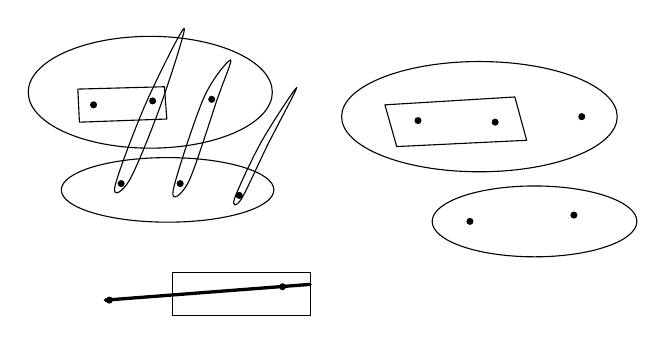
\begin{tikzpicture}[x=1mm,y=1mm,line cap=round,line join=round,font=\scriptsize]
\draw (27.7,-12.9) ellipse[x radius=15.5, y radius=7.1];
\draw (18.5,-12.5) -- (29.5,-12.2) -- (29.8,-16.3) -- (18.7,-16.7) -- cycle;
\node[pt] at (20.5,-14.5) {};
\node[pt] at (28,-14) {};
\node[pt] at (35.5,-13.8) {};
\node[pt] at (24,-24.5) {};
\node[pt] at (31.5,-24.5) {};
\node[pt] at (39,-26) {};
\draw (29.9,-25.3) ellipse[x radius=13.5, y radius=4.1];
\draw plot[smooth cycle, tension=0.55] coordinates {(32,-4.8) (29,-14.6) (25.1,-24) (23.2,-24.9) (27.1,-14.4)};
\draw plot[smooth cycle, tension=0.55] coordinates {(37.9,-8.8) (36.2,-13.8) (32.6,-24.2) (30.6,-25.4) (34.5,-13.6)};
\draw plot[smooth cycle, tension=0.55] coordinates {(46.3,-12.3) (42.6,-19.6) (39.3,-26.4) (38.4,-26.4) (41.8,-19.2)};
\draw (69.5,-16) ellipse[x radius=17.5, y radius=7];
\draw (57.5,-14.5) -- (74,-13.5) -- (75.5,-19) -- (59,-19.8) -- cycle;
\node[pt] at (61.7,-16.5) {};
\node[pt] at (71.5,-16.7) {};
\node[pt] at (82.5,-16) {};
\draw (76.5,-29.3) ellipse[x radius=13, y radius=4.5];
\node[pt] at (68.3,-29.3) {};
\node[pt] at (81.5,-28.5) {};
\draw[very thick] (22,-39.3) -- (48,-37.3);
\node[pt] at (22.5,-39.3) {};
\node[pt] at (44.5,-37.6) {};
\draw (30.5,-35.8) -- (48,-35.8) -- (48,-41.3) -- (30.5,-41.3) -- cycle;
\end{tikzpicture}
\end{document}
